\subsection{Crystalline Rock Samples}
\label{subsec:crystalline}
\Authors{Thomas Fr\"uhwirt, Daniel P\"otschke}

\subsubsection{URL Reiche Zeche Freiberg}
\index{URL Reiche Zeche}

\begin{wrapfigure}{l}{6cm}
\centering
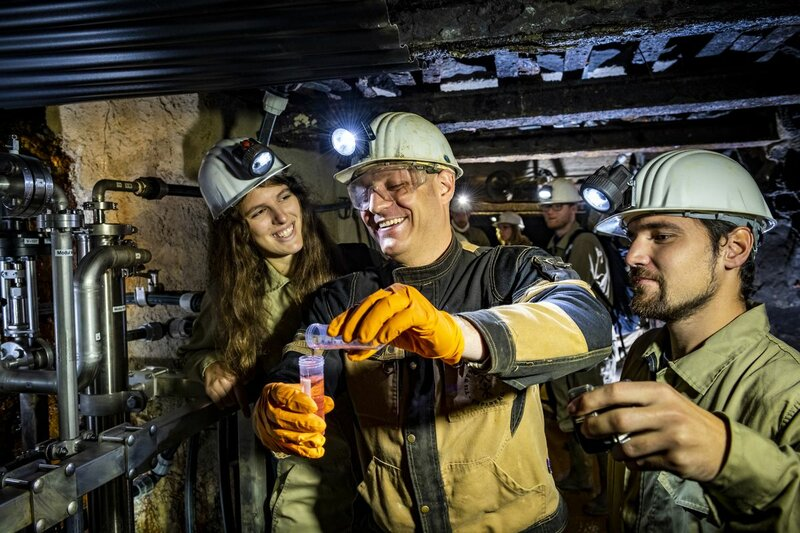
\includegraphics[width=5.9cm]{figures/reiche-zeche.jpg}
\caption{The Reiche Zeche in Freiberg, \cite{ReicheZechePicture}.}
\end{wrapfigure}
The Reiche Zeche mine is located north-east of the city center of Freiberg, Saxony. It operated as a silver mine for several centuries. It became a part of the TU Freiberg 1919 when silver mining definitely was no longer profitable. Nowadays the mine is used as an underground research laboratory (URL) and for teaching purposes. The roughly $4\,\text{km}^2$ sized area is well documented in terms of geology, mineralogy, geophysics and geometry. Draining of the mine is done using the "Rothsch\"onberger Stollen (tunnel)". A detailed overview about the history of the Reiche Zeche can be found in \cite{ReicheZecheHistory}.
%
Due to its long history, the development of new technologies and the importance for the development of the whole region the mining sites and the associated infrastructure are listed as UNESCO world heritage site since 2019.

Current projects are for example dealing with bio-leaching or complex experiments which study the influence of hydro-fracking experiments on the stress state (STIMTEC project).
\index{STIMTEC project}

The Reiche Zeche is equipped with an underground railway system, installed electricity, water and air pressure. The experienced staff and the nearby located mining agency help to successfully conduct experiments in about 150 m depth. 

\subsubsection{Rock material used in the direct shear tests}

\begin{figure}
\begin{subfigure}[c]{0.48\textwidth}
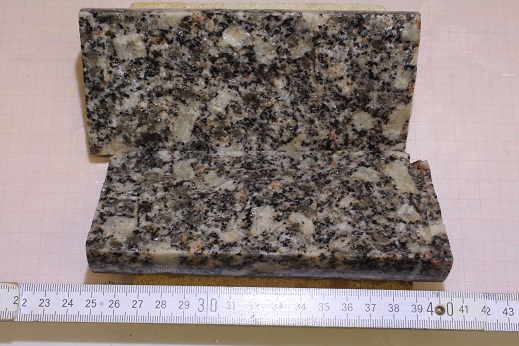
\includegraphics[width=0.99\textwidth]{./figures/ExpRockGranite.JPG}
\subcaption{Granite sample}
\label{fig:RockGranite}
\end{subfigure}
\begin{subfigure}[c]{0.48\textwidth}
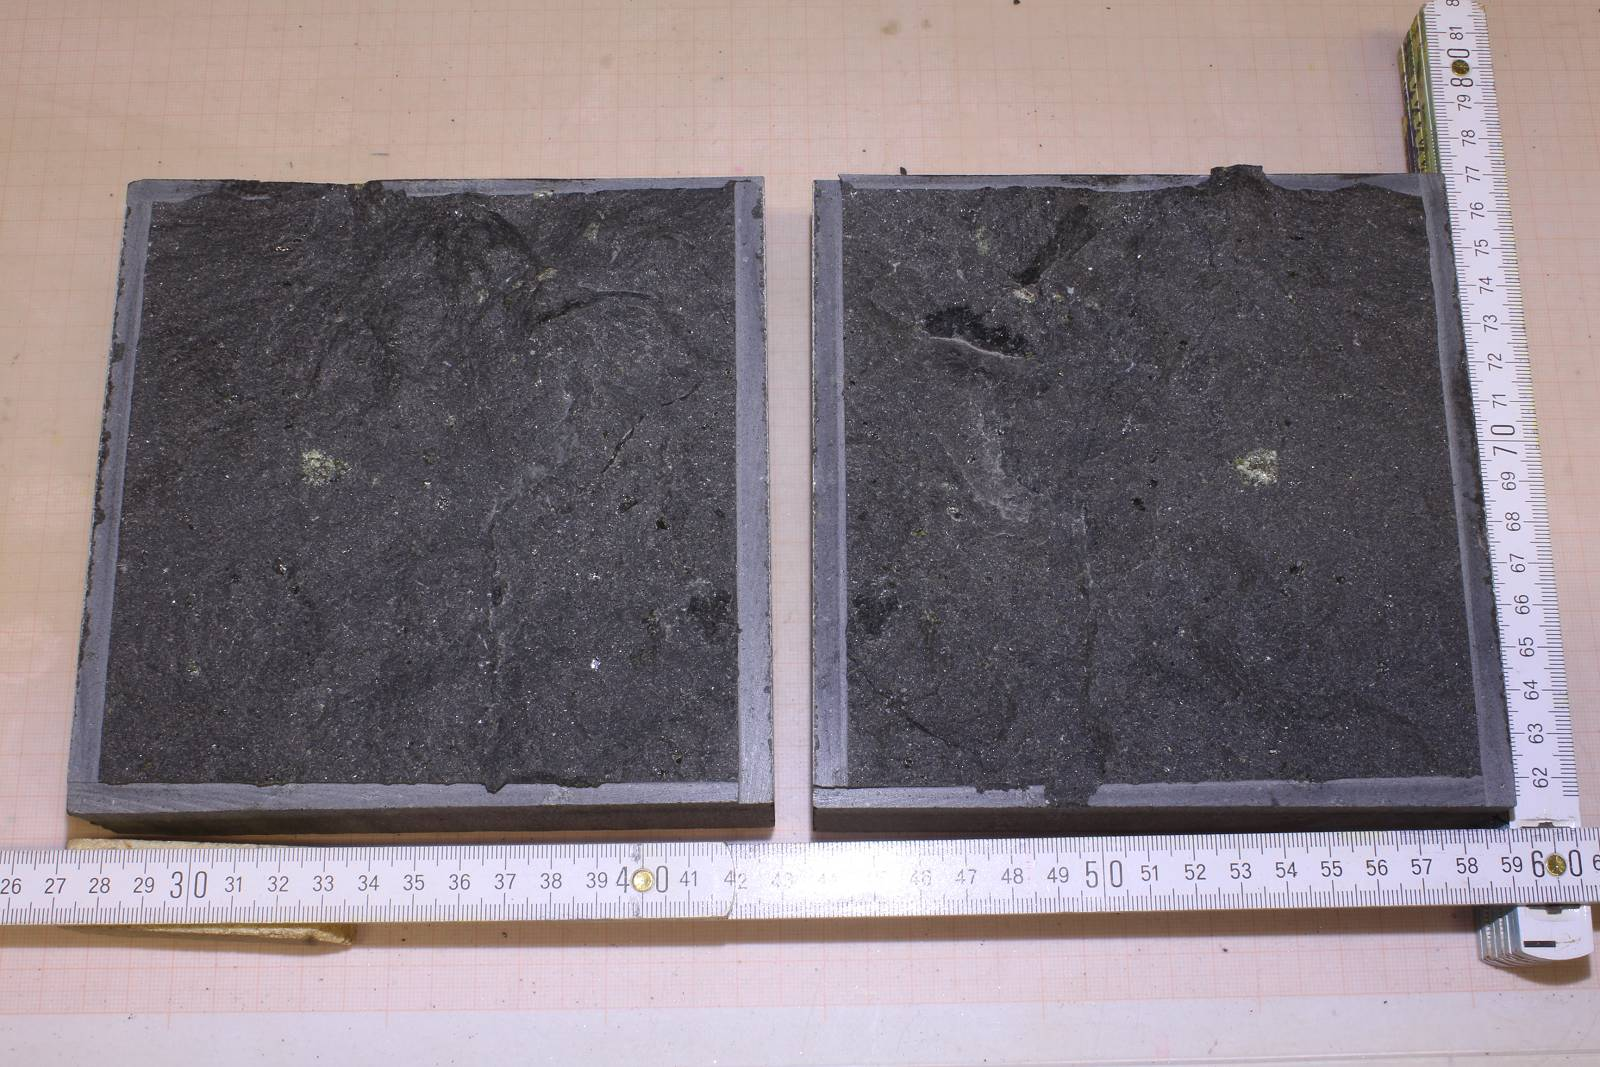
\includegraphics[width=0.99\textwidth]{./figures/ExpRockBasalt.jpg}
\subcaption{Basalt sample}
\label{fig:RockBasalt}
\end{subfigure}
\caption{Crystalline rock samples under investigation}
\end{figure}

Two different crystalline rock \index{crystalline rock} types are used. Granite is a coarse-grained intrusive igneous rock. The grains are on the millimetre to centimetre scale, see Fig. \ref{fig:RockGranite}. The typical main minerals of granites are quartz, feldspar and plagioclase. The used granite origins from Kirchberg, Saxony.
%
Basalt is an fine-grained extrusive igneous rock. It is rich of plagioclase. See Fig. \ref{fig:RockBasalt}. Its origin is V\"olkershausen, Thuringia.
%
Lab tests to evaluate basic rock parameters of the intact rock material have been conducted. The values of the granite and basalt used in the experiments can be found in Tab. \ref{table:MEX7_rockParam}.

\begin{table}[!ht]
\begin{center}
\begin{tabular}{l c r r r}
Parameter & Symbol & Granite & Basalt & Unit\\
\hline
Density & $\rho$ & $2.59$ &3.06 &$\text{g}/\text{cm}^3$\\
Compressive strength & $\sigma_c$ & $120.54$&272.92 &$\text{MPa}   $\\
Tensile strength & $\sigma_t$ & $7.02$&16.61 &$ \text{MPa}   $\\
%static elastic modulus & $E_s$ & $50.00$& &$ \text{GPa}   $\\
Elastic modulus & $E$ & $49.75$&105.46 &$ \text{GPa}   $\\
Poisson's ratio & $\nu$ & 0.26 & 0.26  & -\\
Fracture toughness & $K_I$ & $0.95$& 2.61 &$\text{MPa}\cdot\text{m}^{0.5}$\\
Friction angle (Mohr) & $\phi$ &  $52.5$& 44 &$^\circ$\\
Cohesion & $c$ &  $22.5$& 25.00  &$ \text{MPa}   $\\
Basic friction angle &$\phi_b$ &30 & 31.2 & $^\circ$\\
\end{tabular}
\caption{Rock parameters of granite and basalt used in the direct shear tests.}
\label{table:MEX7_rockParam}
\end{center}
\end{table}

The elastic modulus and the compressive strength were determined using uni-axial compression tests. For the tensile strength a tension test was conducted and the fracture toughness is evaluated by a bending test. The cohesion was determined through a shear test using a saw-cut joint. Ultrasonic measurements were used to determine the Poisson's ratio.
%
The basic friction angles were determined based on \cite{Alejano20121023}. The inner friction angle of basalt is from \cite{Schultz19951} and of granite from \cite{Lanaro2005} and \cite{Ramana2019273}.

\subsubsection{Rock surface scanning}
\index{Rock surface scanning}

Important measurements to characterise a rock surface are surface scans. In the laboratory of the TU Freiberg a white light scanner is used, see Fig. \ref{TUBAFScanner}. It is a non-contact method which uses monochromatic light. A fringe projection is done and surface scans of rock samples with a resolution of about $30-50 \unit{\mu m}$ can be calculated. Further details about the scanning device can be found in \cite{TUBAFScanningDevice}. 

\begin{figure}[!ht]
\centering
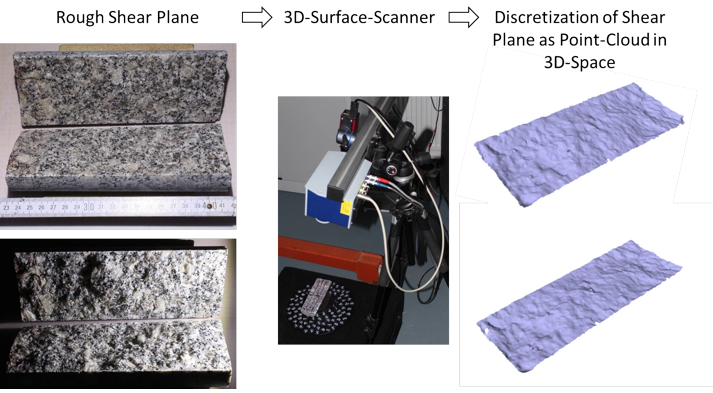
\includegraphics[width=1.4\textwidth, angle=90]{figures/geomint-wp3-12a}
\caption{Surface scanning. A rock surface is digitized using a surface scanning device. The result is a point cloud.}\label{TUBAFScanner}
\end{figure}